\chapter{28 Novembre 2016}
\justify

\newthought{La volta scorsa}, dato un reticolo $L \subseteq \bbC$, avevamo
costruito la funzione di Weierstrass associata $\wp_L (z)$, che soddisfa
un'equazione del tipo $\wp'^2(z) = 4 \wp^3(z) - g_2 \wp(z) - g_3$ dove
$g_2 = 60 s_4$ e $g_3 = 140 s_6$ con $S_n = \sum_{\omega \in L^*}
\omega^{-n}$.

Sia $E: y^2 = 4x^3 - g_2 x - g_3$ (il luogo di zeri in $\bbC^2$) e
consideriamone la chiusura proiettiva $\ol{E} = E \cup \{ (0 : 1 : 0)
\}$.

\begin{notazione}
  Con $\ol{E}(\bbK)$ si intendono i punti $\bbK$-razionali di $\ol{E}$,
  ovvero i punti di $\bbP^2 \bbC$ per le quali il rapporto tra le
  coordinate è un numero di $\bbK$, ovvero
  $\ol{E}(\bbK) = \{ (x : y : z) \in \ol{E} \mid \frac{x}{y},
  \frac{y}{z} \in \bbK \}$
\end{notazione}

\newthought{Consideriamo la mappa} $F: T = \sfrac{\bbC}{L} \rar \ol{E}$
dal toro relativo al reticolo $L$ alla chiusura proiettiva della
cubica. $F$ è definita da $z \mapsto (\wp(z) : \wp'(z) : 1)$ dove questa
espressione ha senso. Quando invece $z$ è un polo di $\wp$, si può usare
un'altra espressione per la mappa, definita sul polo, ma che coincida
con quella fornita sui punti in cui si intersecano gli aperti di
definizione.

\notamargine{Ad esempio si può considerare l'espressione
  $$\lbr{1 : \frac{\wp'(z)}{\wp(z)} : \frac{1}{\wp(z)}}$$

  Notiamo che stiamo trattando $T$ come una varietà olomorfa e ciò che
  stiamo facendo è definire una mappa tra varietà su alcune carte
}

\begin{proposizione}
  $F$ è una biggezione tra $T$ ed $\ol{E}(\bbC)$ (ed è olomorfa)
\end{proposizione}
\notamargine{Ricordiamo che tutte le funzioni meromorfe su $T$ sono
  $\bbC(\wp(z), \wp'(z))$, mentre le fuznioni meromorfe pari su $T$ sono
  esattamente $\bbC(\wp(z))$}
\begin{proof}
  Sia $p \in \ol{E}(\bbC)$. Distinguiamo in due casi:
  \begin{itemize}
  \item Se $p = (0 : 1 : 0)$ ok per costruzione (significa che la $\wp$
    ha un polo e quindi come unico punto abbiamo $z = 0 \in T$)
  \item Se $p \in E(\bbC)$ (nella parte affine della cubica) sia $p =
    (x_0, y_0)$

    Consideriamo allora $\wp(z) - x_0$ che è una funzione ellittica pari
    non costante che ha due zeri (con molteplicità). Se $z_0$ è uno zero
    lo è anche $- z_0$ (dove i punti si intendono sul
    toro). Distinguiamo in due casi a seconda della derivata nel punto:
    \begin{itemize}
    \item Se $\wp'(z_0) = 0$ allora $z_0$ è uno zero doppio e deve
      quindi coincidere con $-z_0$ sul toro, ovvero nel piano ho
      solamente quattro possibilità: sono la metà dei generatori del
      parallelogramma fondamentale del toro.
      
      \notamargine{Nella figura qui sotto è disegnato il
        parallelogramma fondamentale di un toro. Sono evidenziati con
        un pallino vuoto i punti che corrispondono alla metà dei
        generatori del parallelogrammo.

        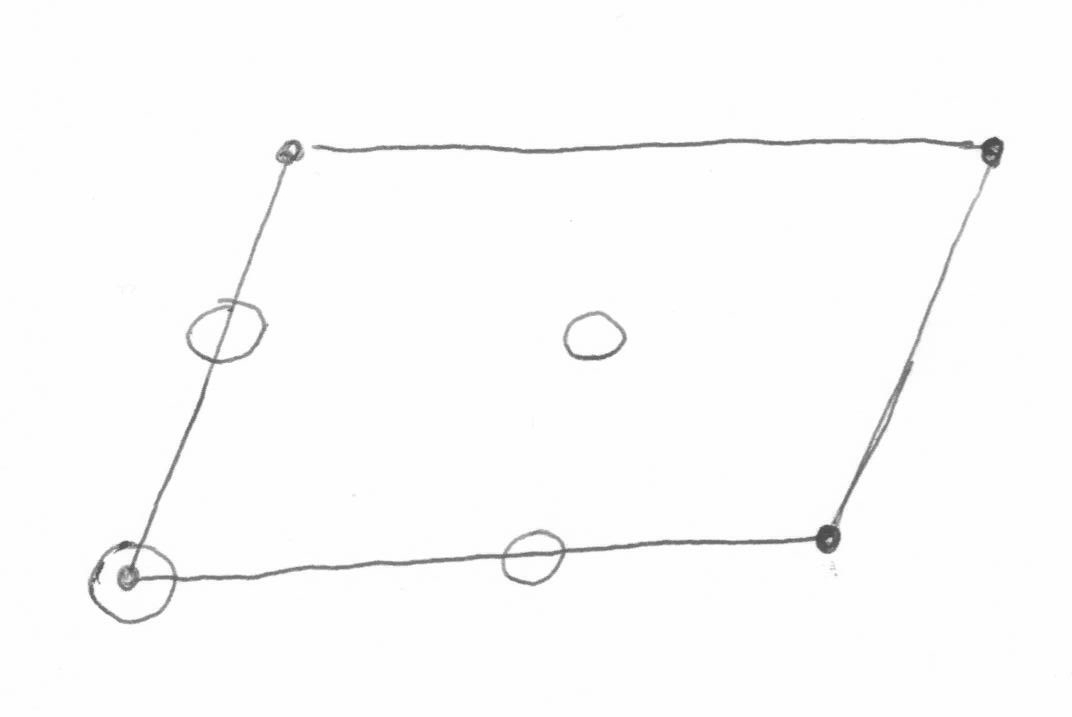
\includegraphics[width=3cm]{lezione-161128-fig1}}

      Allora si ha un solo punto tale che $4x_0^3 - g_2 x_0 - g_3 = 0 (=
      \wp'(z_0))$ e quindi anche questo caso è ok
    \item Se $\wp'(z_0) \neq 0$ allora si ha $z_0 \neq - z_0$ in $T$ e
      quindi $\wp'(z_0) = - \wp'(-z_0)$ poiché la $\wp'$ è
      dispari. Siamo allora nel caso $4x_0^3 - g_2 x_0 - g_3 = \alpha
      \neq 0$ e per avere $y = \pm \sqrt{\alpha}$ posso usare $z_0$ ed
      anche $-z_0$, ovvero ancora una volta la tesi è verificata.
    \end{itemize}
  \end{itemize}

  Per quanto riguarda l'olomorfia, basta aggiungere che la mappa fornita
  $z \mapsto (\wp(z) : \wp'(z) : 1)$ è ovviamente olomorfa tra $T$ e
  $\bbP^2 \bbC$
\end{proof}

\begin{osservazione}
  Notiamo però che se mi viene dato un polinomio di terzo grado nella
  forma $y^2 = 4x^3 - g_2 x - g_3$ non so ancora dire se venga da un
  toro oppure no. Se viene da un toro allora ho la corrispondenza
  biunivoca (proposizione precedente) $\sfrac{\bbC}{L} \leftrightarrow T$
\end{osservazione}

\begin{osservazione}
  Se abbiamo un polinomio in due variabili $f(x, y) = 0$ abbiamo una
  superficie di Riemman, ma non avevamo dimostrato (nel caso delle
  cubiche) la connessione, che in generale non è ovvia.

  Nel caso delle cubiche ciò segue dalla proposizione appena dimostrata.
\end{osservazione}

\paragraph{Altra dimostrazione della connessione} Dimostriamo ancora una
volta che $\ol{E}(\bbC)$ è connesso, iniziando dalla connessione di
$E(\bbC)$ (spazio dei punti affini)

% $x \mapsto 4x^3 - g_2 x - g_3$

La funzione di proiezione $E(\bbC) \rar \bbC$ definita da $(x, y) \mapsto x$ 
diventa un rivestimento tolte le tre radici $\alpha, \beta, \gamma$ del
polinomio $4x^3 - g_2 x - g_3$.

\notamargine{L'idea è che, tolte le radici, abbiamo un rivestimento di
  grado due. I punti del rivestimento si riescono a connettere ``facendo
  dei giri attorno alle radici''}

\begin{center}
  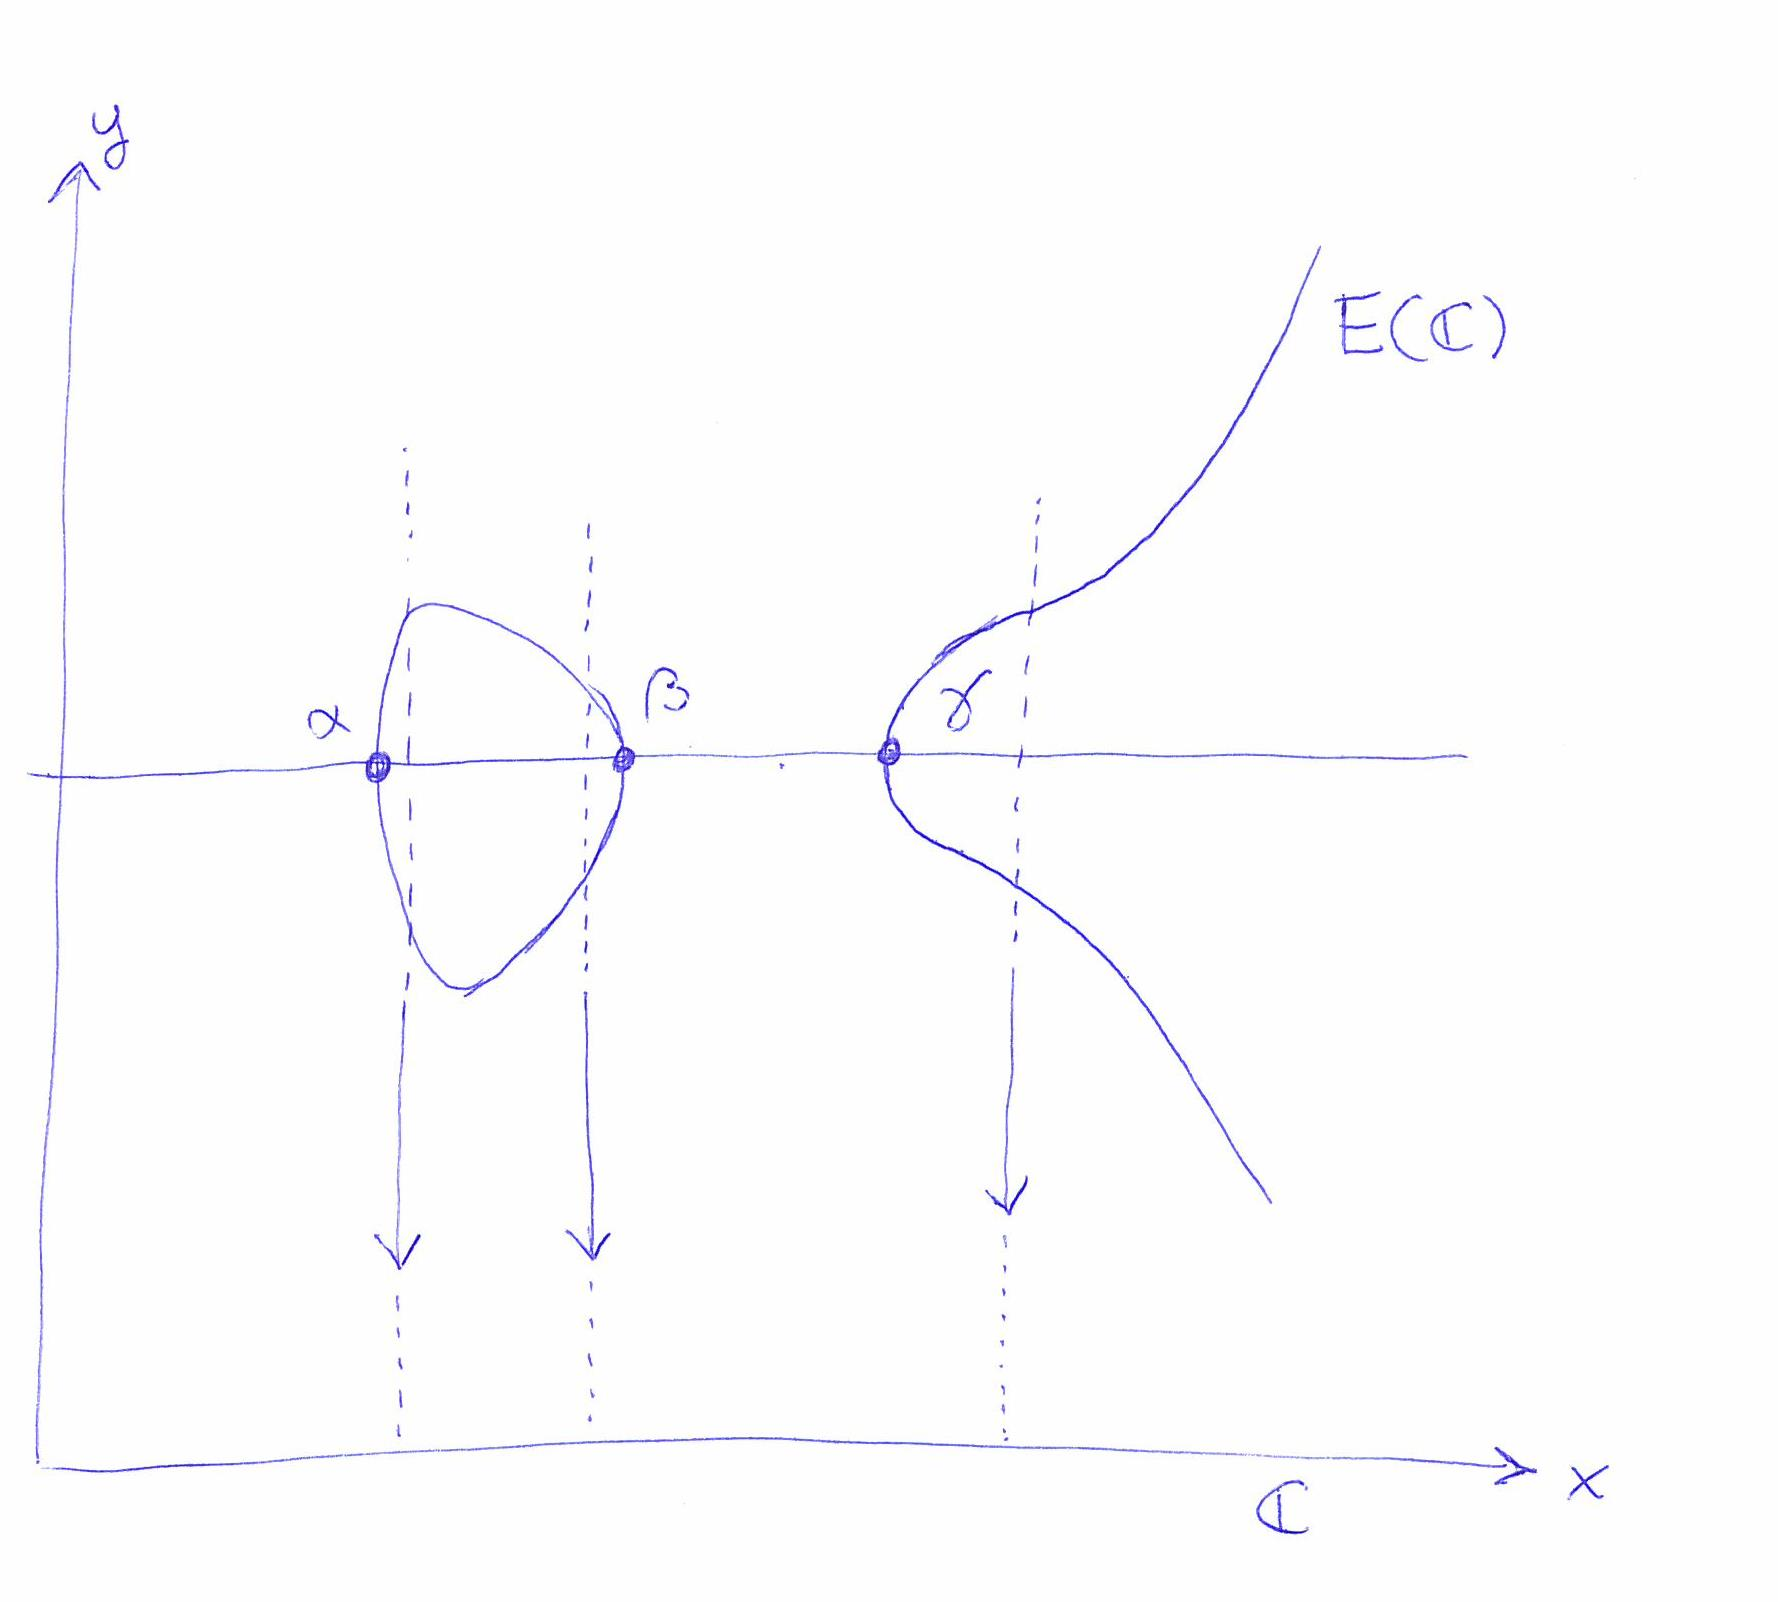
\includegraphics[width=8cm]{lezione-161128-fig1bis}
\end{center}

\notamargine{Per dimostrare che è un rivestimento, possiamo utilizzare
  il fatto che le proiezioni sono mappe aperte e che il numero di punti
  $(x, y) \in E(\bbC)$ che si proiettano su $x$ sono, per
  $x \neq \alpha, \beta, \gamma$, esattamente due, ovvero quelli che
  risolvono $y^2 = 4x^3 - g_2 x - g_3$ con $x$ fissato}

Ovviamente si ha che, avendo il rivestimento grado due, o è connesso,
oppure ha due componenti connesse. Ora, se facciamo un cammino tra due
punti $x_0$ ed $x_1$ del $\bbC$ ``che viene ricoperto'' posso sollevare
il cammino, perché ho un rivestimento. Per mostrare la connessione del
rivestimento basta quindi dimostrare che la fibra di $x_0 \neq \alpha,
\beta, \gamma$ ``è connessa'', ovvero ho un cammino che connette i due
elementi della fibra.

\begin{center}
  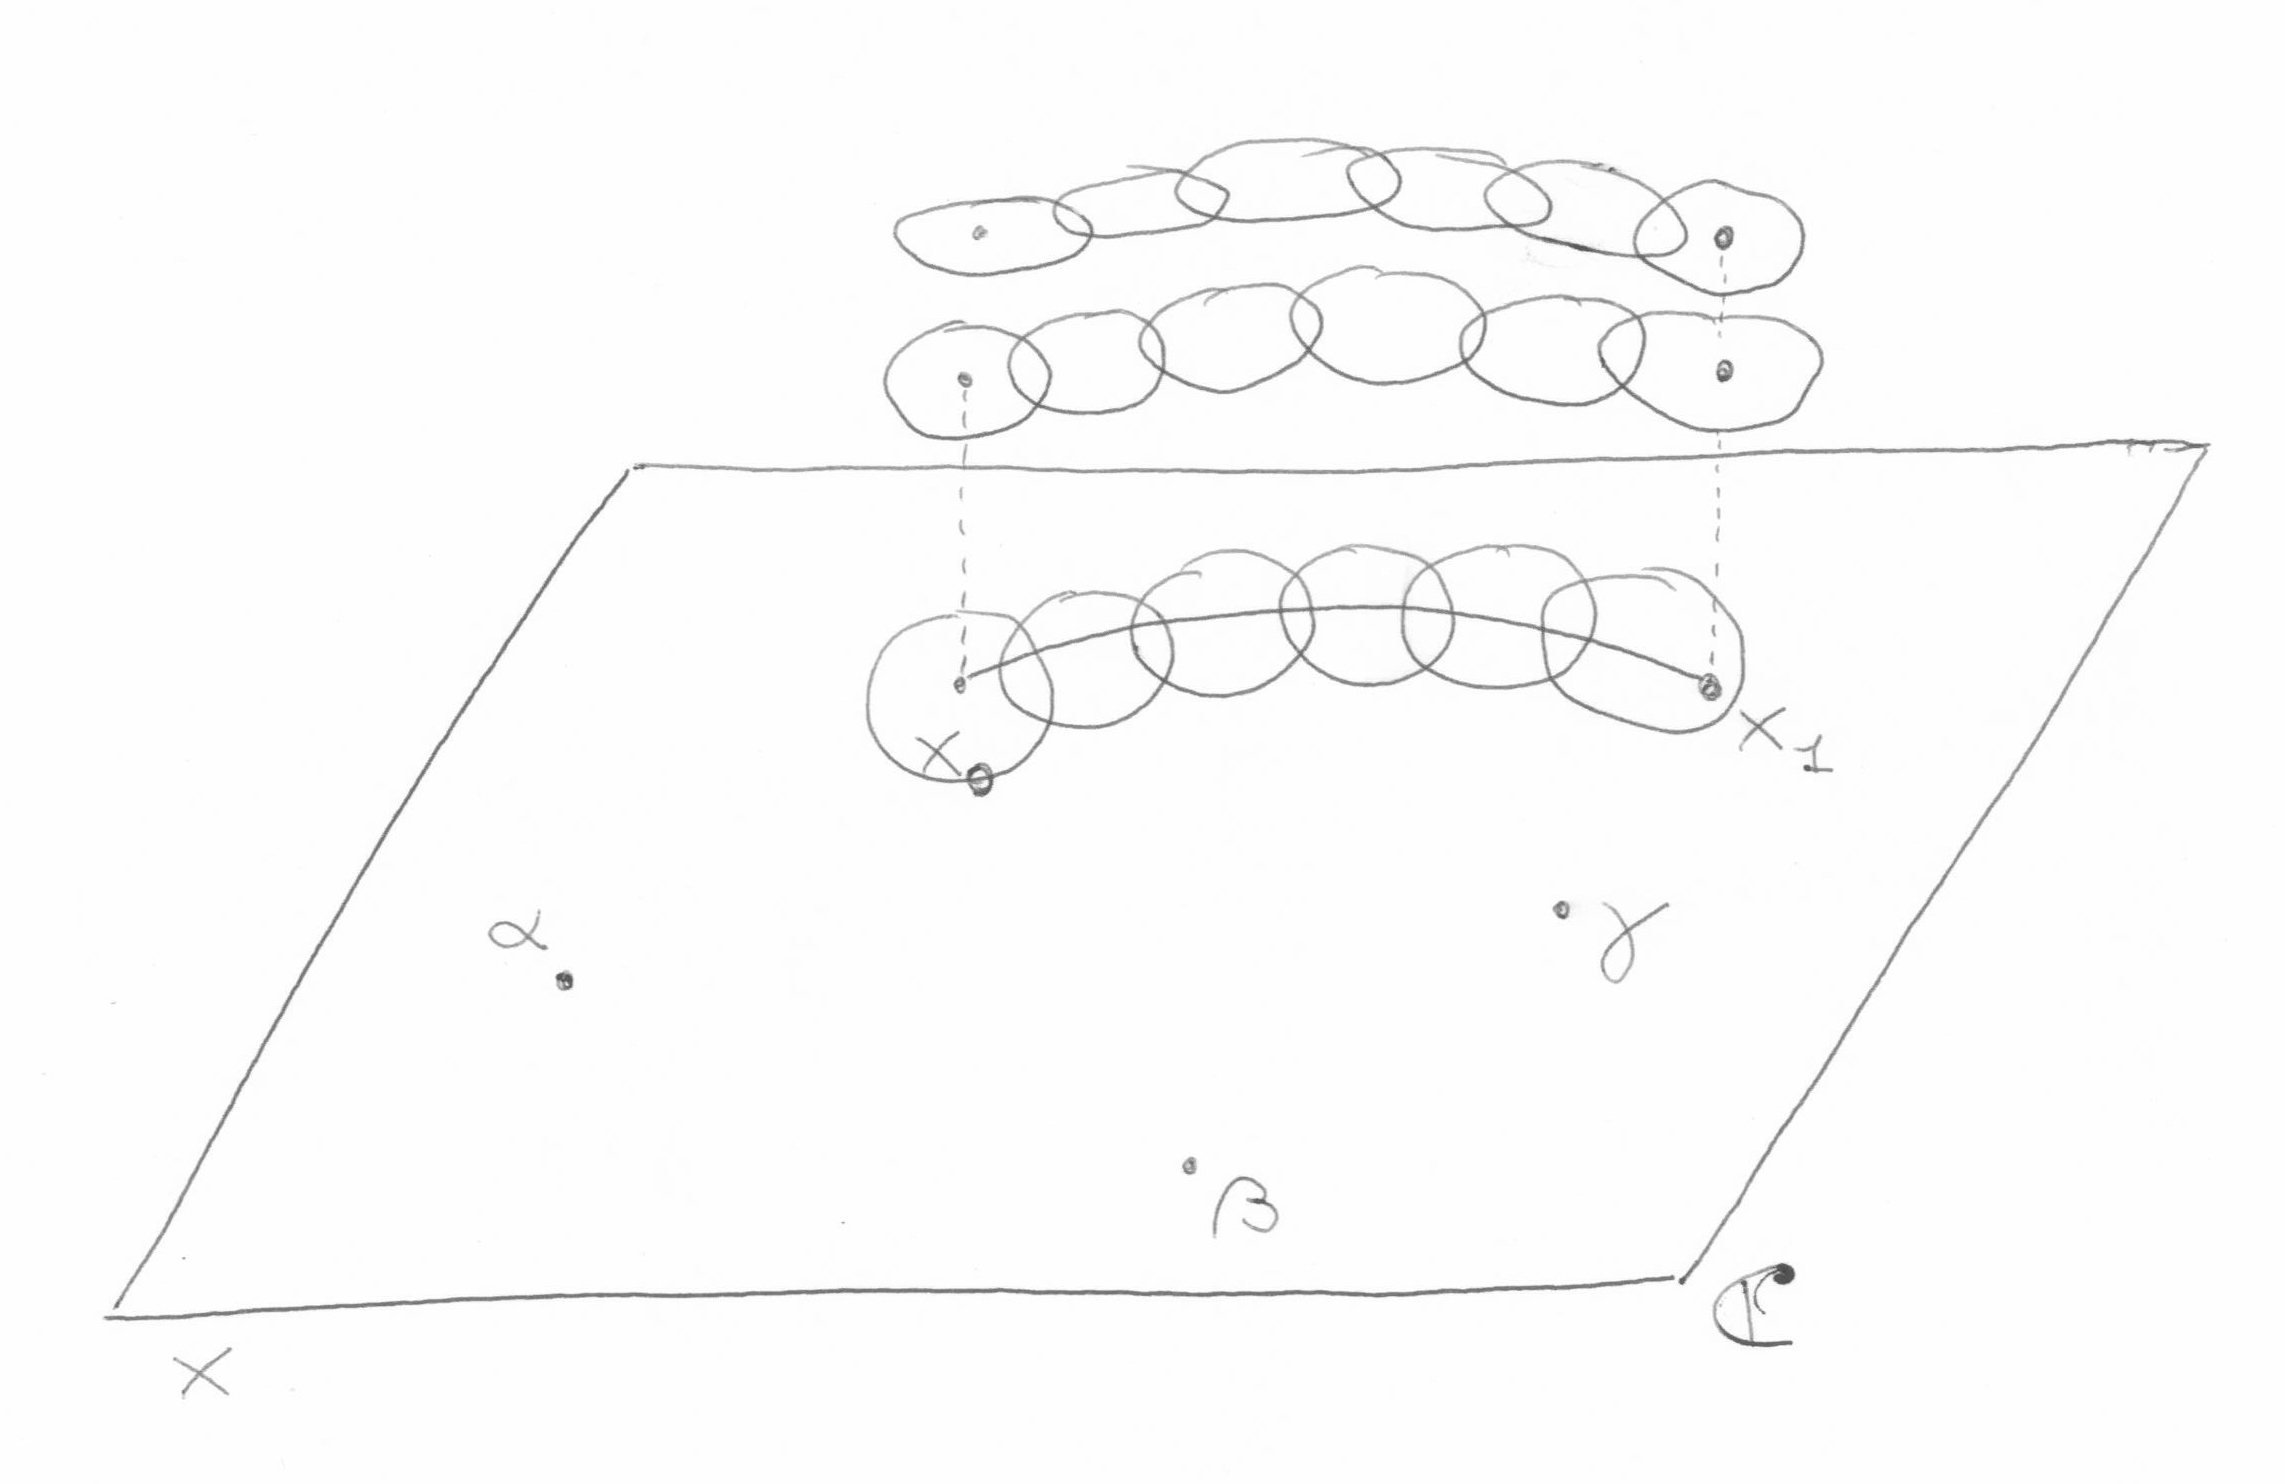
\includegraphics[width=8cm]{lezione-161128-fig2}
\end{center}

Ciò è molto semplice da fare con la radice quadrata: prendiamo infatti
un punto $x_0$ vicino ad $\alpha$. Allora si ha che
$\sqrt{f(x)} = (x - \alpha)^{\frac{1}{2}} \cdot g(x)$ con $g(x)$
olomorfa vicino ad $\alpha$ (poiché siamo lontani da $\beta$ e da
$\gamma$)

Scegliamo una determinazione della radice e facciamo un giro attorno ad
$\alpha$ tornando sulla fibra di $x_0$ ma con valore del segno cambiato.

\notamargine{In particolare si può scegliere un cerchio di raggio
  piccolo (cammino $t \mapsto x_0 + \rho e^{2\pi i t}$) e fare
  esplicitamente il conto ricordando che $z^\frac{1}{2}$ è definito con
  una determinazione di $e^{\log(\frac{1}{2} z)}$}

\section{Cubiche di $\bbP^2\bbC$}
Consideriamo tutte le cubiche in $\bbP^2\bbC$: esse sono definite da
un'equazione omogenea di grado tre $F(x, y, z) = 0$. Mostreremo ora che
nel caso la cubica è parametrizzabile se e solo se è singolare.

\notamargine{Ricordiamo che per parametrizzazione intendiamo una
  isomorfismo birazionale con $\bbP^1$, ovvero una funzione razionale
  $f: \bbP^1 \rar E$ che si intende definita da quasi tutti i punti di
  $\bbP^1$ a quasi tutti i punti di $E$. (Quasi tutti significa tutti
  tranne al più un numero finito)}

\subsection{Caso singolare}
Sappiamo che esiste un punto singolare (ovvero che appartiene alla curva
e su cui tutte le derivate parziali dell'equazione definente la curva si
annullano, ovvero in cui la dimensione del tangente è due).

Allora, se intersechiamo la cubica con il fascio di rette passante per
il punto singolare otteniamo la parametrizzazione (per esercizio
mostrare che ogni retta incontra esattamente un punto della chiusura
proiettiva della cubica e che, ovviamente, dato ogni punto della cubica
esiste una retta che passa per lui e per il punto singolare). La cubica
è quindi parametrizzabile.

\notamargine{Inoltre di punti singolari ne ha al più uno: se ve ne
  fossero due $p, q$ posso tracciare la retta passante per $p$ e per
  $q$, che intersecherebbe la cubica con molteplicità quattro.}

\subsection{Caso non singolare}
In ogni cubica c'è sempre un punto di flesso (ovvero dove l'hessiano si
annulla). Usando una proiettività si può mandare il flesso nel punto
all'infinito $(0 : 1 : 0)$.

\notamargine{L'Hessiano in questo caso è il determinante della matrice
  hessiana del polinomio che definisce la cubica, ovvero
  $\Det (\frac{\partial F}{\partial x_i \partial x_j})_{i, j = 1, 2, 3}$

  Il polinomio hessiano ha, per un facile conto, grado $3 (d-2)$, dove
  $d$ è il grado della curva $F$, oppure è identicamente nullo.
  Nel primo caso, per il teorema di Bèzout, esistono punti di $\bbP^2$
  su cui esso si annulla assieme all'equazione di $F$, ovvero esistono
  punti di $F$ di flesso (e sappiamo anche che sono $3 (d - 2) d$
  contati con molteplicità)}

Facendo i conti con il flesso all'infinito e con tangente al flesso la
retta $\{ z = 0 \}$ ottengo un'equazione simile a quella di Weierstrass
a cui si arriva con alcune manipolazioni algebriche:
$y^2 = 4 x^3 - a x - b$.

Se poi effettuiamo la trasformazione $x \mapsto \lambda^2 x$ e $y
\mapsto \lambda^3 y$ con $\lambda \neq 0$ allora si ottiene $y^2 = 4 x^3
- \frac{a}{\lambda^4} x - \frac{b}{\lambda^6}$.

Posso quindi scegliere $\lambda$ in modo da far scomparire un parametro.

\begin{osservazione}
  Non sappiamo ancora che ogni cubica viene da un toro, quindi non
  potevamo dire a priori che lo spazio delle cubiche ha un solo
  parametro.
\end{osservazione}

Che succede se al posto di un reticolo $L$ ne prendiamo uno omotetico
$\lambda L$ con $\lambda \in \bbC^*$? Le funzioni $g_2$ e $g_3$ si
trasformano nel seguente modo:
$ g_2 \mapsto \frac{g_2}{\lambda^4} ,\quad g_3 \mapsto
\frac{g_3}{\lambda^6}$ e quindi l'equazione della cubica diventa:
$E_{\lambda L}: y^2 = 4x^3 - \frac{g_2}{\lambda^4} x -
\frac{g_3}{\lambda^6}$

Quali sono le funzioni razionali di $a$ e di $b$ che rimangono
invarianti per trasformazioni omotetiche? Sicuramente vi è
$\frac{a^3}{b^2}$.
\notamargine{Per esercizio si può dimostrare che ogni funzione razionale
  invariante per omotetia di $a$ e di $b$ si scrive come funzione
  razionale di $\frac{a^3}{b^2}$}

Dato un reticolo $L$, lo scriviamo come $\bbZ \tau + \bbZ$ con $\tau \in
\cH$ (semipiano superiore) a meno di rotomotetie del piano.

\begin{proposizione}
  $\frac{g_2^3}{g_3^2}$ è una funzione di $\tau$ non costante e meromorfa
\end{proposizione}

Per quanto riguarda la meromorfia, si può notare che, definita la somma
$$S_n = \sum_{(r, s) \in \bbZ^2 \setminus \{(0, 0)\}} \frac{1}{(r \tau
  + s)^n}$$ essa converge per $n \ge 2$ e definisce una funzione olomorfa
di $\tau$. Segue quindi che, se $S_3$ non è identicamente nulla, si ha
che $\frac{g_2^3}{g_3^2} = \frac{S_2^3(\tau)}{S_3^2(\tau)}$ per
definizione e quindi la succitata funzione è meromorfa.

\notamargine{Per verificare la convergenza assoluta della sommatoria per
  $n > 2$ si può maggiorare la serie dei valori assoluti con l'opportuno
  integrale in due variabili. Per il caso $n=2$ non saprei...}

Inoltre, se trovassimo due reticoli $L_1$ ed $L_2$ in cui valga
rispettivamente
$$g_3(L_1) = 0, g_2(L_1) \neq 0$$
$$g_2(L_2) = 0, g_3(L_2) \neq 0$$
ne seguirebbe che la funzione non è costante.

Si possono a tal proposito considerare i reticoli $\tau = i$ e
$\tau = \zeta_3$:
\begin{itemize}
\item ($\tau = i$) Sia $L_1 = \bbZ[i]$. Allora si nota che $i L_1 = L_1$
  e quindi si ha $g_2(i L_1) = g_2(L_1)$ e per omogeneità
  $g_3(L_1) = g_3(i L_1) = i^{-6} g_3(L_1)$ da cui segue $g_3(L_1) = 0$.

  Inoltre $g_2 \neq 0$, altrimenti il polinomio definente avrebbe radici
  multiple (segue direttamente dall'equazione del polinomio).

\item ($\tau = \zeta_3$) Sia $L_2 = \bbZ[\zeta_3]$ e notiamo che
  $\zeta_3 L_2 = L_2$ che implica $g_2(L_2) = g_2(\zeta_3 L_2) =
  \zeta_3^4 g_2(L_2) = \zeta_3 g_2(L_2)$ e quindi $g_2(L_2) = 0$
\end{itemize}

